\chapter{Proposed Methodology}
\label{Chapter3}
\lhead{Chapter 3. \emph{Proposed Methodology}}

\section{Problem Summary}

High-fidelity thermal image synthesis from RGB photographs is essential for applications in surveillance, medical diagnostics, and precision agriculture, yet is hindered by the prohibitive cost of LWIR cameras and the scarcity of paired RGB--thermal datasets. Existing image translation frameworks (pix2pix, CycleGAN) lack domain-specific physical priors --- they neither enforce the smooth spatial gradients dictated by the heat diffusion PDE nor match the low-frequency-dominant spectral signature of real thermal images. Furthermore, the original LiquidGAN framework suffers from a flat 128-dimensional latent bottleneck that destroys spatial detail, producing blurry outputs despite using a Neural ODE. PC-LiquidGAN addresses all three limitations by combining a spatial ODE-UNet generator, physics-constrained losses, and FFT spectral supervision within an adversarial training framework.

\section{Overview}

PC-LiquidGAN is a physics-constrained generative adversarial network for RGB-to-thermal image synthesis. The overall framework, illustrated in Figure~\ref{fig:arch}, consists of:
\begin{itemize}
    \item An \textbf{ODE-UNet Generator} $G$ that maps RGB images to thermal images via continuous spatial ODE dynamics and skip-connection-based spatial reconstruction.
    \item A \textbf{Liquid Neural Network Discriminator} $D$ that classifies thermal images as real or synthesised using CNN features refined by a liquid cell with learnable time constants.
    \item A composite loss function $\mathcal{L}_G$ that combines adversarial, pixel-wise reconstruction, heat diffusion PDE, and FFT spectral terms.
\end{itemize}

\begin{figure}[htbp]
    \centering
    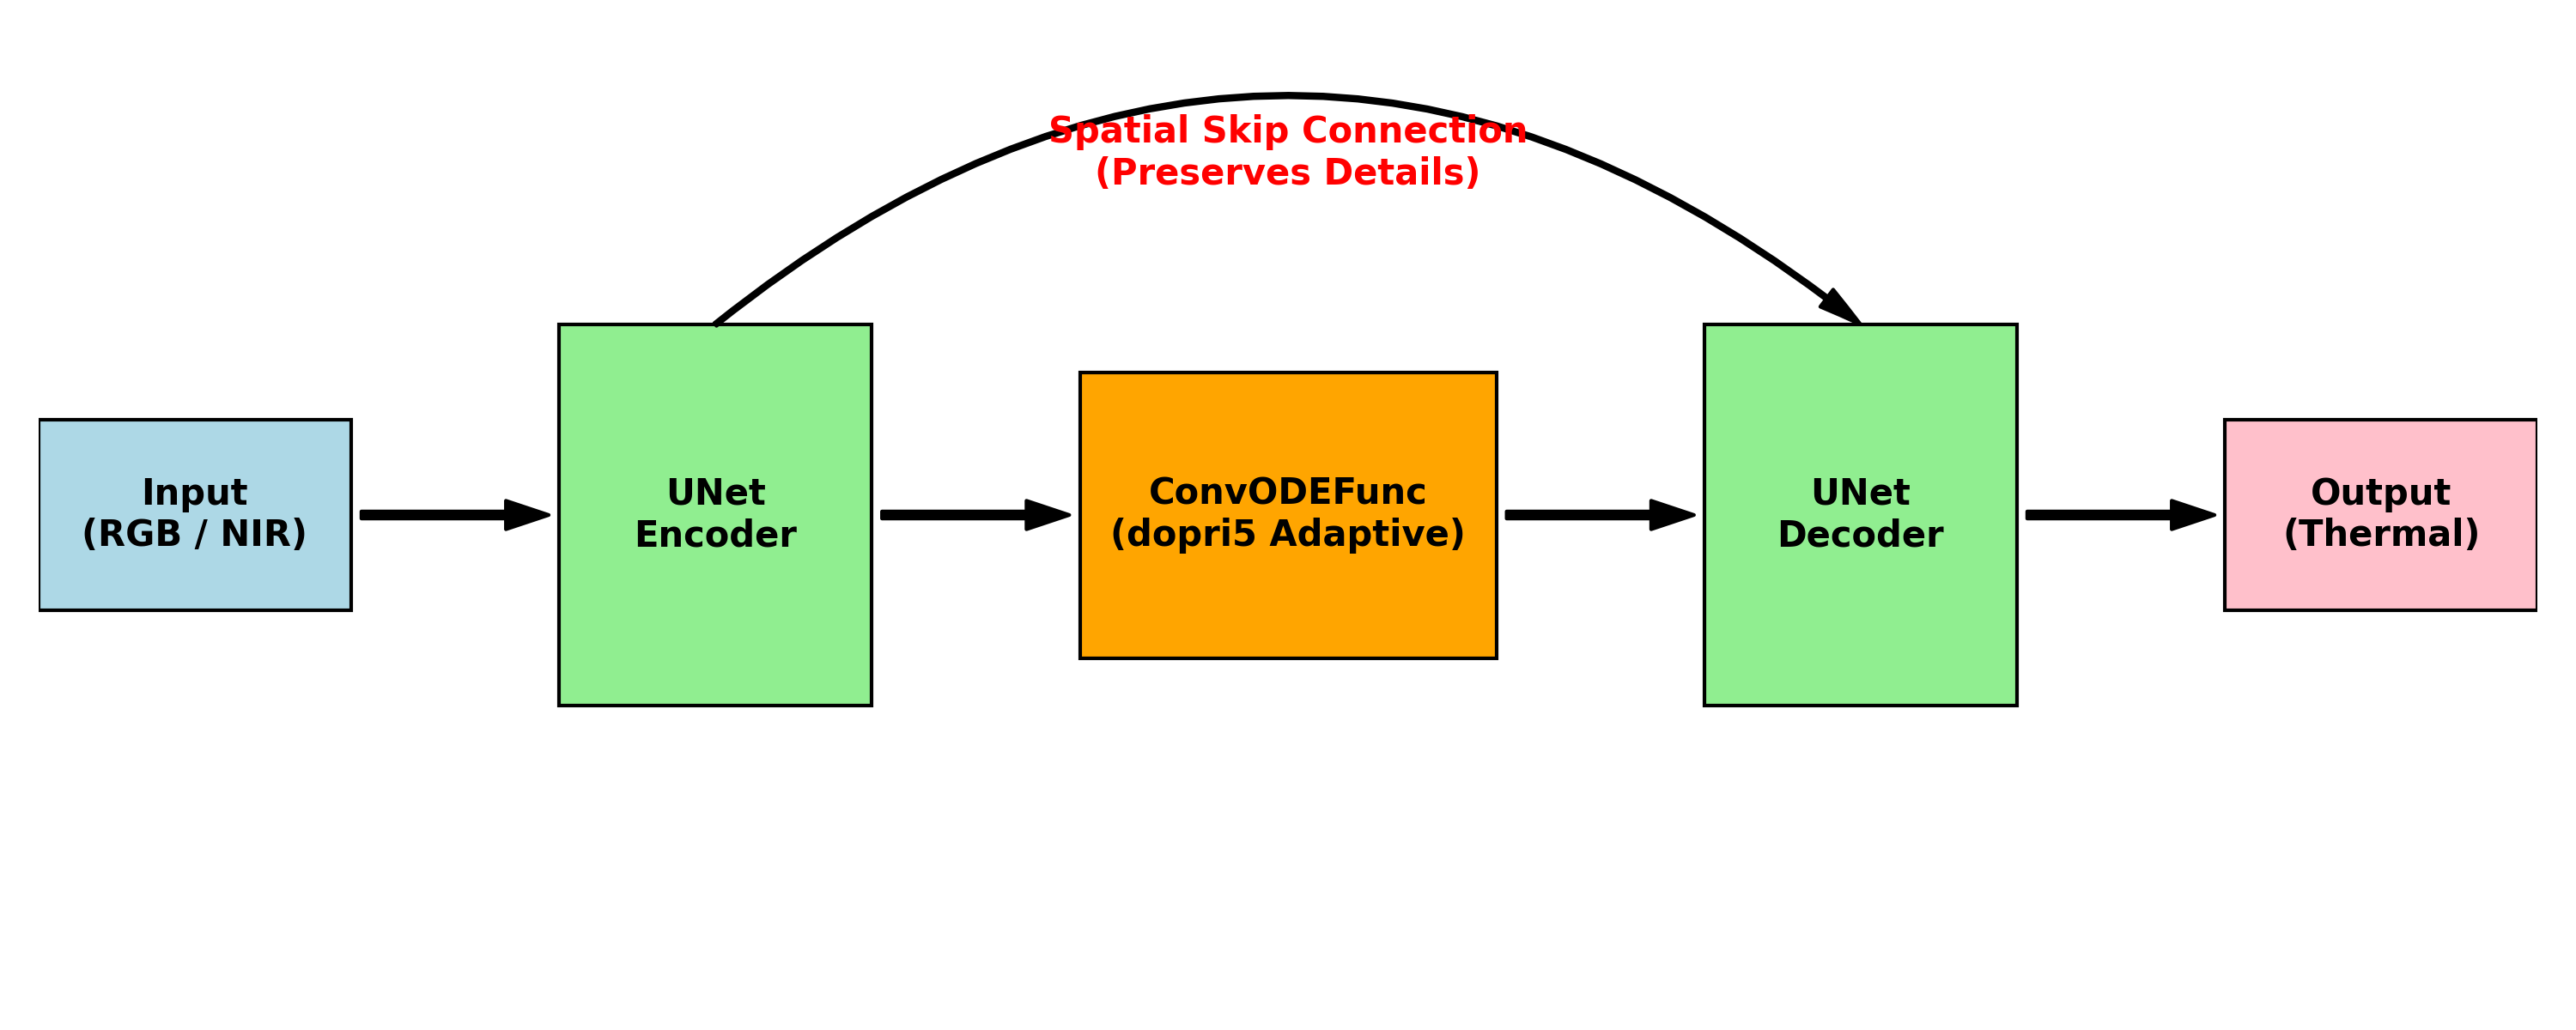
\includegraphics[width=\linewidth]{architecture.png}
    \caption{High-level architecture of PC-LiquidGAN. The ODE-UNet generator maps RGB images to thermal images. The LNN discriminator provides adaptive discrimination feedback. Physics and spectral losses enforce thermodynamic plausibility.}
    \label{fig:arch}
\end{figure}

\section{Physics-Constrained Thermal Modelling}

\subsection{Governing Equation}

The temperature distribution $T(\mathbf{x}, t)$ in a thermally conductive medium evolves according to the heat diffusion PDE:
\begin{equation}
    \frac{\partial T(\mathbf{x}, t)}{\partial t} = \alpha \nabla^2 T(\mathbf{x}, t)
    \label{eq:heat}
\end{equation}
where $\alpha$ is the thermal diffusivity constant (material property) and $\nabla^2 = \frac{\partial^2}{\partial x^2} + \frac{\partial^2}{\partial y^2}$ is the 2D Laplacian operator. For a physically valid thermal image, the residual $R(\mathbf{x}, t) = \frac{\partial T}{\partial t} - \alpha \nabla^2 T$ should be zero everywhere.

\subsection{Heat Diffusion Flux Loss}

We approximate the temporal derivative $\partial T/\partial t$ as the difference between the generated and real thermal images (assuming unit time between the RGB observation and the corresponding thermal steady-state):
\begin{equation}
    \mathcal{L}_{flux} = \frac{1}{N} \sum_{\mathbf{x}} \left( \hat{T}(\mathbf{x}) - T(\mathbf{x}) - \alpha \nabla^2 \hat{T}(\mathbf{x}) \right)^2
    \label{eq:flux}
\end{equation}
The discrete 2D Laplacian is computed via convolution with the $3\times3$ kernel:
\begin{equation}
    K_{\nabla^2} = \begin{bmatrix} 0 & 1 & 0 \\ 1 & -4 & 1 \\ 0 & 1 & 0 \end{bmatrix}
\end{equation}

\subsection{Energy Conservation Loss}

Total thermal energy $E(t) = \iint T(\mathbf{x}, t)\, d\mathbf{x}$ is conserved in a closed system. We enforce this per-sample as:
\begin{equation}
    \mathcal{L}_{energy} = \left( \frac{1}{HW}\sum_{i,j} \hat{T}_{i,j} - \frac{1}{HW}\sum_{i,j} T_{i,j} \right)^2
    \label{eq:energy}
\end{equation}

\subsection{Gradient Smoothness Loss}

Real thermal images exhibit spatially smooth gradients due to heat diffusion. We additionally penalise sharp spatial discontinuities:
\begin{equation}
    \mathcal{L}_{smooth} = \frac{1}{HW}\sum_{i,j} \left( |\hat{T}_{i,j+1} - \hat{T}_{i,j}| + |\hat{T}_{i+1,j} - \hat{T}_{i,j}| \right)
\end{equation}

\subsection{Combined Physics Loss}

\begin{equation}
    \mathcal{L}_{physics} = \lambda_{flux} \mathcal{L}_{flux} + \lambda_{energy} \mathcal{L}_{energy} + \lambda_{smooth} \mathcal{L}_{smooth}
    \label{eq:physics}
\end{equation}
with $\lambda_{flux} = 0.5$, $\lambda_{energy} = 0.25$, $\lambda_{smooth} = 0.1$.

\section{Frequency-Domain Spectral Loss}

Real thermal images are low-frequency dominant: solutions to the heat diffusion PDE (Eq.~\ref{eq:heat}) attenuate high spatial frequencies exponentially. Pixel-space losses (L1, L2) do not enforce this spectral structure. The spectral loss directly penalises differences in the FFT magnitude spectra:

\begin{equation}
    \mathcal{L}_{spec} = \| \left|\mathcal{F}(\hat{T})\right| \odot W - \left|\mathcal{F}(T)\right| \odot W \|_F^2
    \label{eq:spectral}
\end{equation}
where $\mathcal{F}(\cdot)$ denotes the 2D FFT, $|\cdot|$ the magnitude, and $W$ is a Gaussian low-frequency emphasis mask:
\begin{equation}
    W_{i,j} = \exp\left( -\frac{(i - H/2)^2 + (j - W/2)^2}{2\sigma^2} \right), \quad \sigma = 32
\end{equation}

\section{Total Generator Objective}

The complete generator loss combines all four terms:
\begin{equation}
    \mathcal{L}_G = \lambda_{adv} \mathcal{L}_{adv} + \lambda_{L1} \mathcal{L}_{L1} + \lambda_{phys} \mathcal{L}_{physics} + \lambda_{spec} \mathcal{L}_{spec}
    \label{eq:total}
\end{equation}
with $\lambda_{adv} = 1.0$, $\lambda_{L1} = 10.0$, $\lambda_{phys} = 0.1$, $\lambda_{spec} = 0.05$.

\section{Training Stabilisation}

GAN training is notoriously unstable. We employ five complementary stabilisation techniques:

\begin{enumerate}
    \item \textbf{Instance Noise:} Gaussian noise $\sigma: 0.1 \to 0$ is added to all discriminator inputs during the first 50 epochs. This blurs the discriminator's decision boundary early in training, preventing it from becoming immediately overconfident.
    \item \textbf{Label Smoothing:} Real labels are set to 0.9 (not 1.0) and fake labels to 0.05 (not 0.0), preventing the discriminator from producing saturated probabilities.
    \item \textbf{L1 Warmup (10 epochs):} During the first 10 epochs, the generator is trained exclusively with L1 reconstruction loss. This provides a useful initialisation before adversarial pressure is applied.
    \item \textbf{2:1 Generator-to-Discriminator Update Ratio:} The generator is updated twice per discriminator step to compensate for the discriminator's natural advantage.
    \item \textbf{Gradient Clipping:} Gradient norms are clipped to 1.0 for both $G$ and $D$ to prevent exploding gradients during Neural ODE adjoint backpropagation.
\end{enumerate}

\section{Differences from the Base LiquidGAN Paper}

Table~\ref{tab:diff} summarises the differences between PC-LiquidGAN and the base LiquidGAN framework.

\begin{table}[htbp]
\centering
\caption{Comparison between Base LiquidGAN and Proposed PC-LiquidGAN.}
\label{tab:diff}
\begin{tabular}{lll}
\toprule
\textbf{Component} & \textbf{Base LiquidGAN} & \textbf{PC-LiquidGAN (Ours)} \\
\midrule
Generator & Flat-latent Neural ODE & ODE-UNet (spatial ConvODE + skip connections) \\
ODE Solver & Fixed RK4 (4 steps) & Adaptive dopri5 ($\sim$44 steps) \\
Discriminator & LNN (retained) & LNN (retained) \\
Physics Loss & None & Heat diffusion PDE + energy conservation \\
Spectral Loss & None & FFT with Gaussian low-freq mask \\
Bottleneck & 128-dim flat vector & $64 \times 16 \times 16$ spatial feature map \\
Skip Connections & None & 4-level encoder-to-decoder \\
\bottomrule
\end{tabular}
\end{table}